% Chapter 3

\chapter{Results} % Main chapter title

\label{Chapter3} % For referencing the chapter elsewhere, use \ref{Chapter1} 

\lhead{Chapter 3. \emph{Results}} % This is for the header on each page - perhaps a shortened title

%----------------------------------------------------------------------------------------

\section{FHN}



\begin{figure}[htbp]
 
  \centering
    \includegraphics[width=0.49\textwidth]{Figures/PA_FCM_c_02.eps} 
	\includegraphics[width=0.49\textwidth]{Figures/PA_FCM_v_7.eps} 

	
    \rule{35em}{0.5pt}
  \caption[Parameter Analysis, FCM]{FHN simulated FCM brain graphs, parameter analysis, $v=7[m/s]$ on the left and $c=0.2$ on the right }
  \label{fig:Parameter Analysis, FCM}
 	
\end{figure}  



\begin{figure}[htbp]
 
  \centering
	 \includegraphics[width=0.49\textwidth]{Figures/cor_FCM_sim.eps} 
   	 \includegraphics[width=0.49\textwidth]{Figures/cor_FCM_exp.eps} 

    \rule{35em}{0.5pt}
  \caption[Best correlated FHN simulation, FCM]{Best correlated FHN simulation of FCM brain graph with $c=0.2$, $v=7 [m/s]$ and $r=0.60$ (on the left) and empirical FCM obtained from fMRI-BOLD. $\rho_{e,s} = 0.43$} 
    \label{fig:Best correlated FHN simulation, FCM}
 	
\end{figure}  



\begin{figure}[htbp]
 
  \centering
	 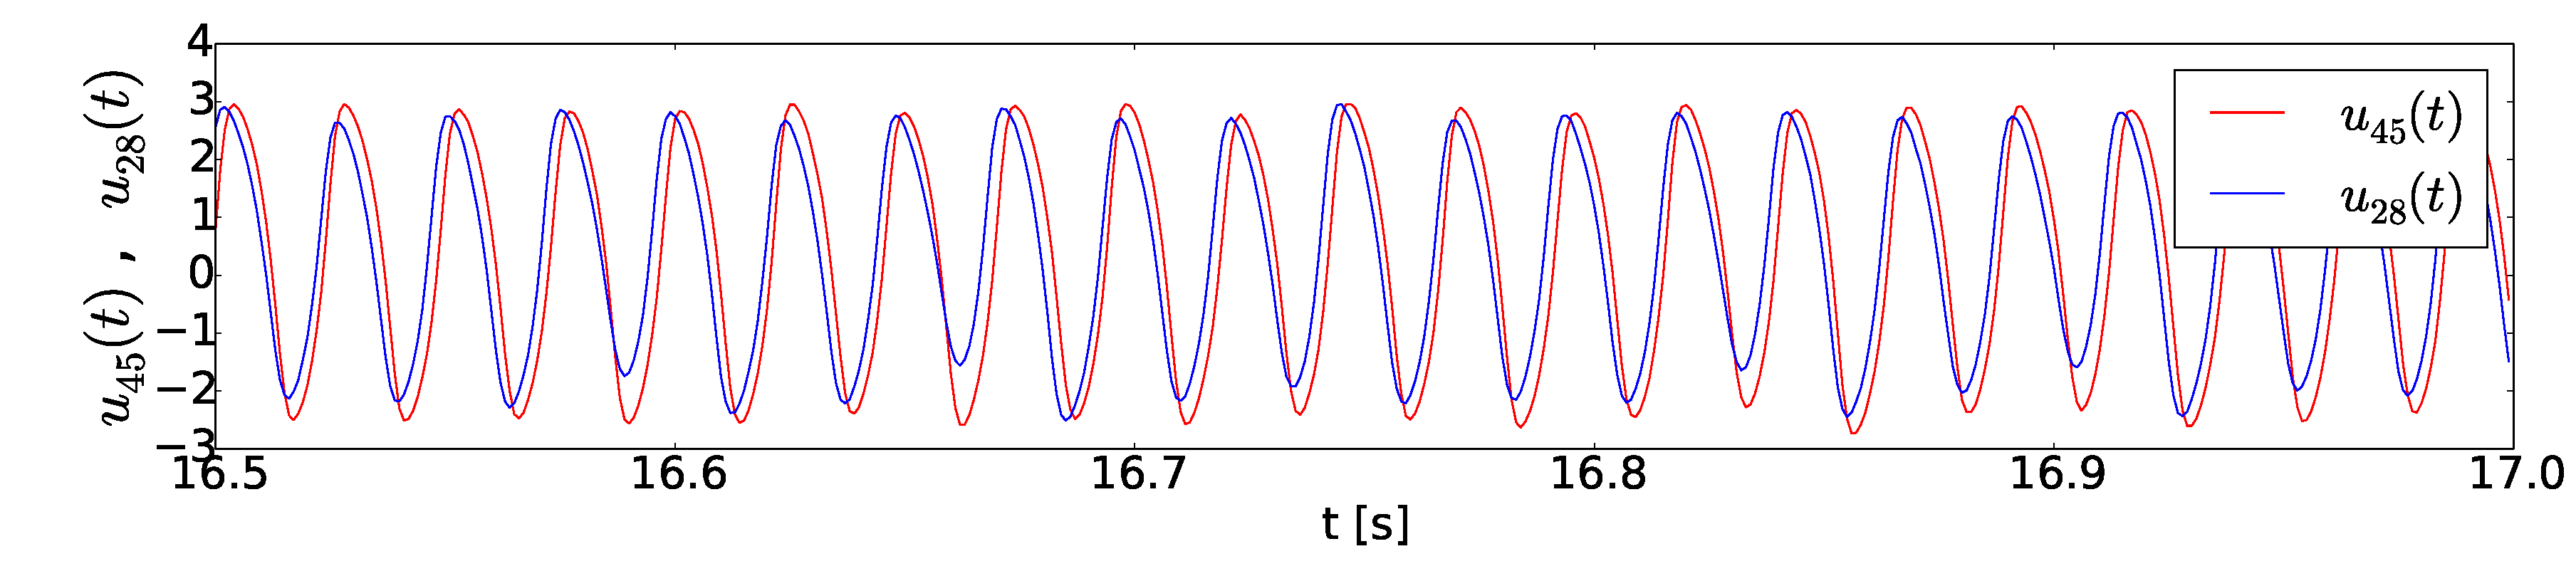
\includegraphics[width=\textwidth]{Figures/cor_FCM_sim_no_best.eps} 
   	 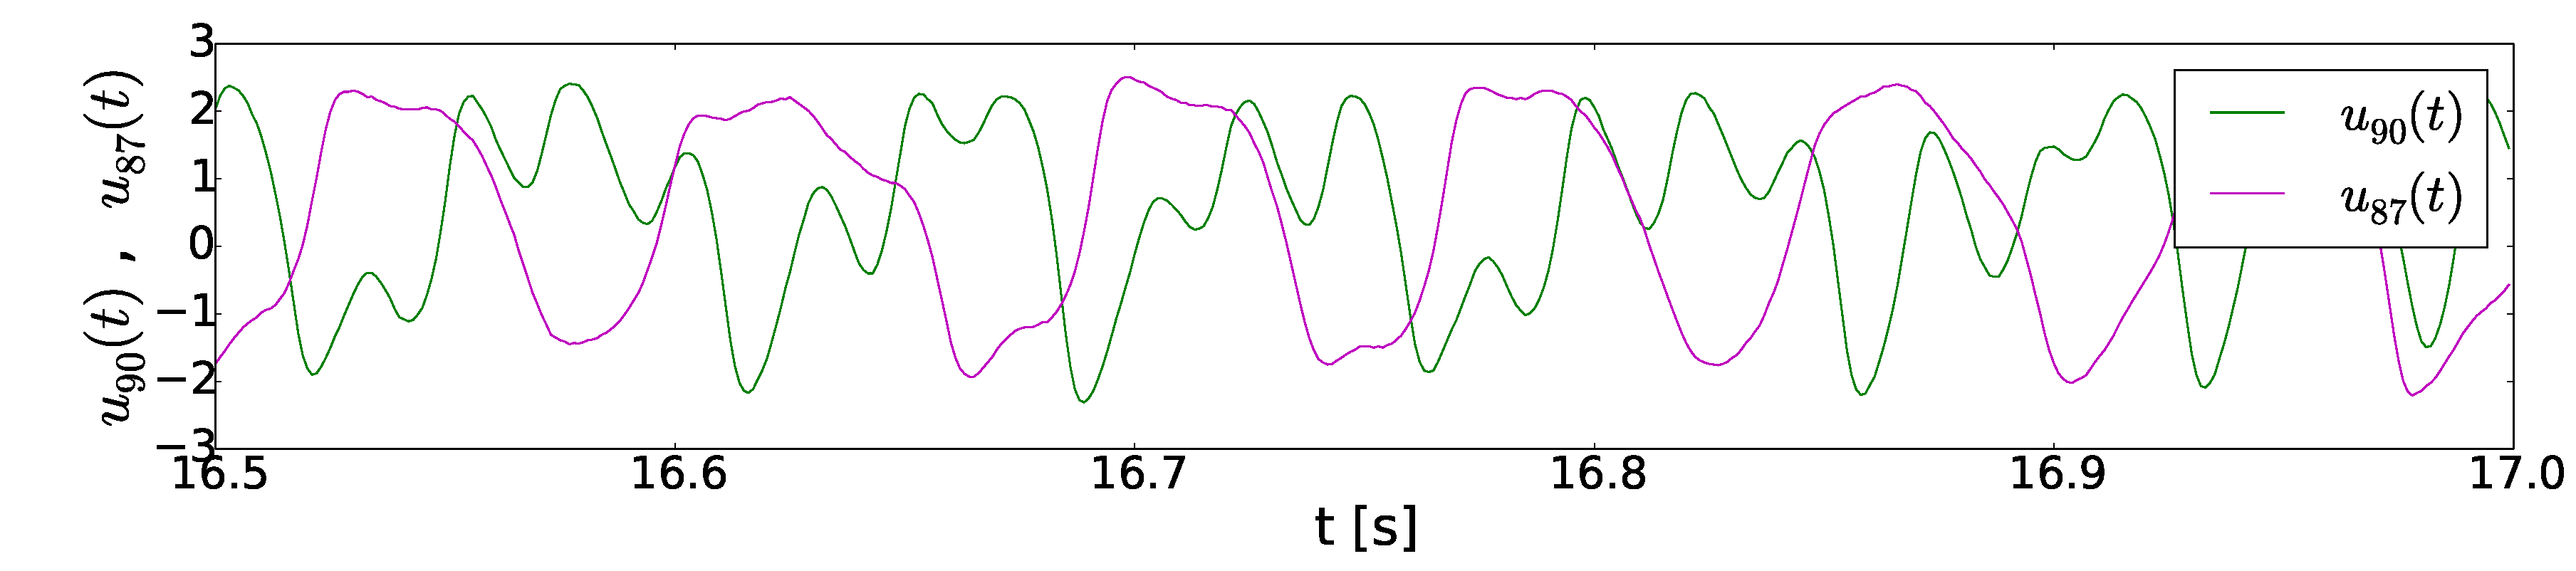
\includegraphics[width=\textwidth]{Figures/cor_FCM_sim_no_worst.eps} 

    \rule{35em}{0.5pt}
  \caption[Neural Activity Node Dynamics, FCM]{Simulated neuronal activity of highly (at top, $\rho_{45,28}=0.88$) and poorly (at bottom, $\rho_{90,87}=0.13$) correlated node couples. Both nodes are chosen from the simulated correlation matrix of FCM in previous figure ($c=0.2$, $v=7 [m/s]$, $r=0.60$).} 
    \label{fig:Neural Activity Node Dynamics, FCM}
 	
\end{figure} 


\begin{figure}[htbp]
 
  \centering
	 \includegraphics[width=0.8\textwidth]{Figures/FFT_FCM.eps} 
   	 %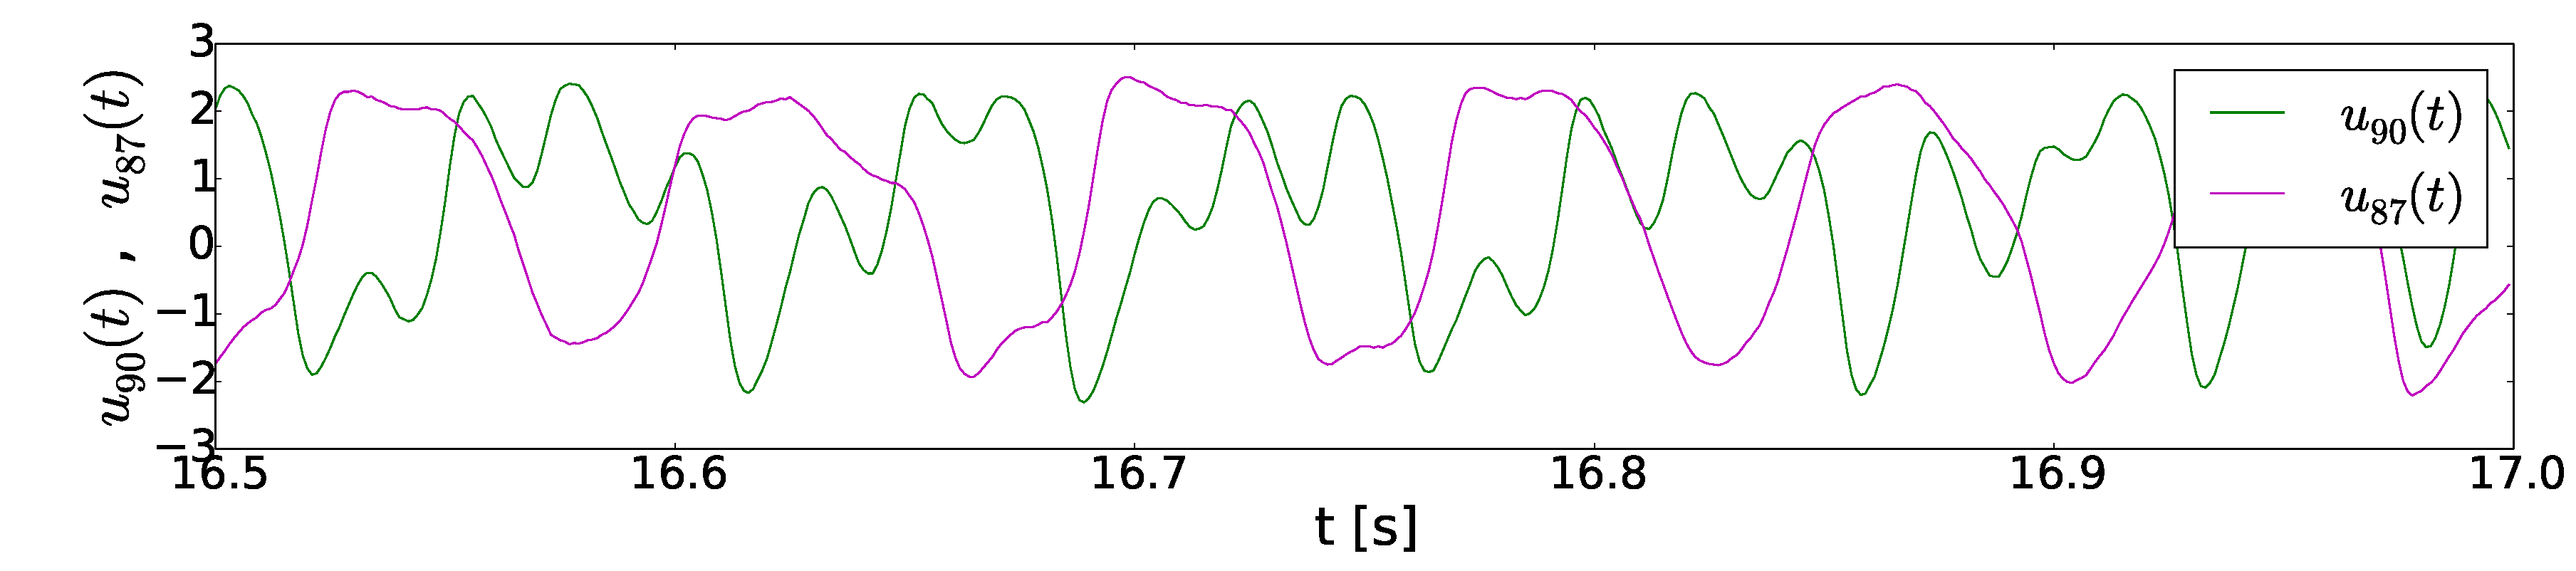
\includegraphics[width=\textwidth]{Figures/cor_FCM_sim_no_worst.eps} 

    \rule{35em}{0.5pt}
  \caption[3D Fourier Transform, FHN, FCM]{3D illustration of fast fourier transform of neuronal activity oscillations corresponding to $N=90$ nodes in FCM simulation with parameters given in Fig.3.2.} 
    \label{fig:3D Fourier Transform, FHN, FCM}
 	
\end{figure}  
 



%\subsection{ACM}

\begin{figure}[htbp]
 
  \centering
    \includegraphics[width=0.49\textwidth]{Figures/PA_ACM_c_03.eps} 
	\includegraphics[width=0.49\textwidth]{Figures/PA_ACM_v_6.eps} 

	
    \rule{35em}{0.5pt}
  \caption[Parameter Analysis, ACM]{FHN simulated ACM brain graphs, parameter analysis, $v=6[m/s]$ on the left and $c=0.3$ on the right }
  \label{fig:Parameter Analysis, ACM}
 	
\end{figure} 





\begin{figure}[htbp]
 
  \centering
	 \includegraphics[width=0.49\textwidth]{Figures/cor_ACM_sim.eps} 
   	 \includegraphics[width=0.49\textwidth]{Figures/cor_ACM_exp.eps} 

    \rule{35em}{0.5pt}
  \caption[Best correlated FHN simulation, ACM]{Best correlated FHN simulation of ACM brain graph with $c=0.3$, $v=6 [m/s]$ and $r=0.50$ (on the left) and empirical ACM obtained from DW-MRI. $\rho_{e,s} = 0.43$} 
    \label{fig:Best correlated FHN simulation, ACM}
 	
\end{figure}



\begin{figure}[htbp]
 
  \centering
	 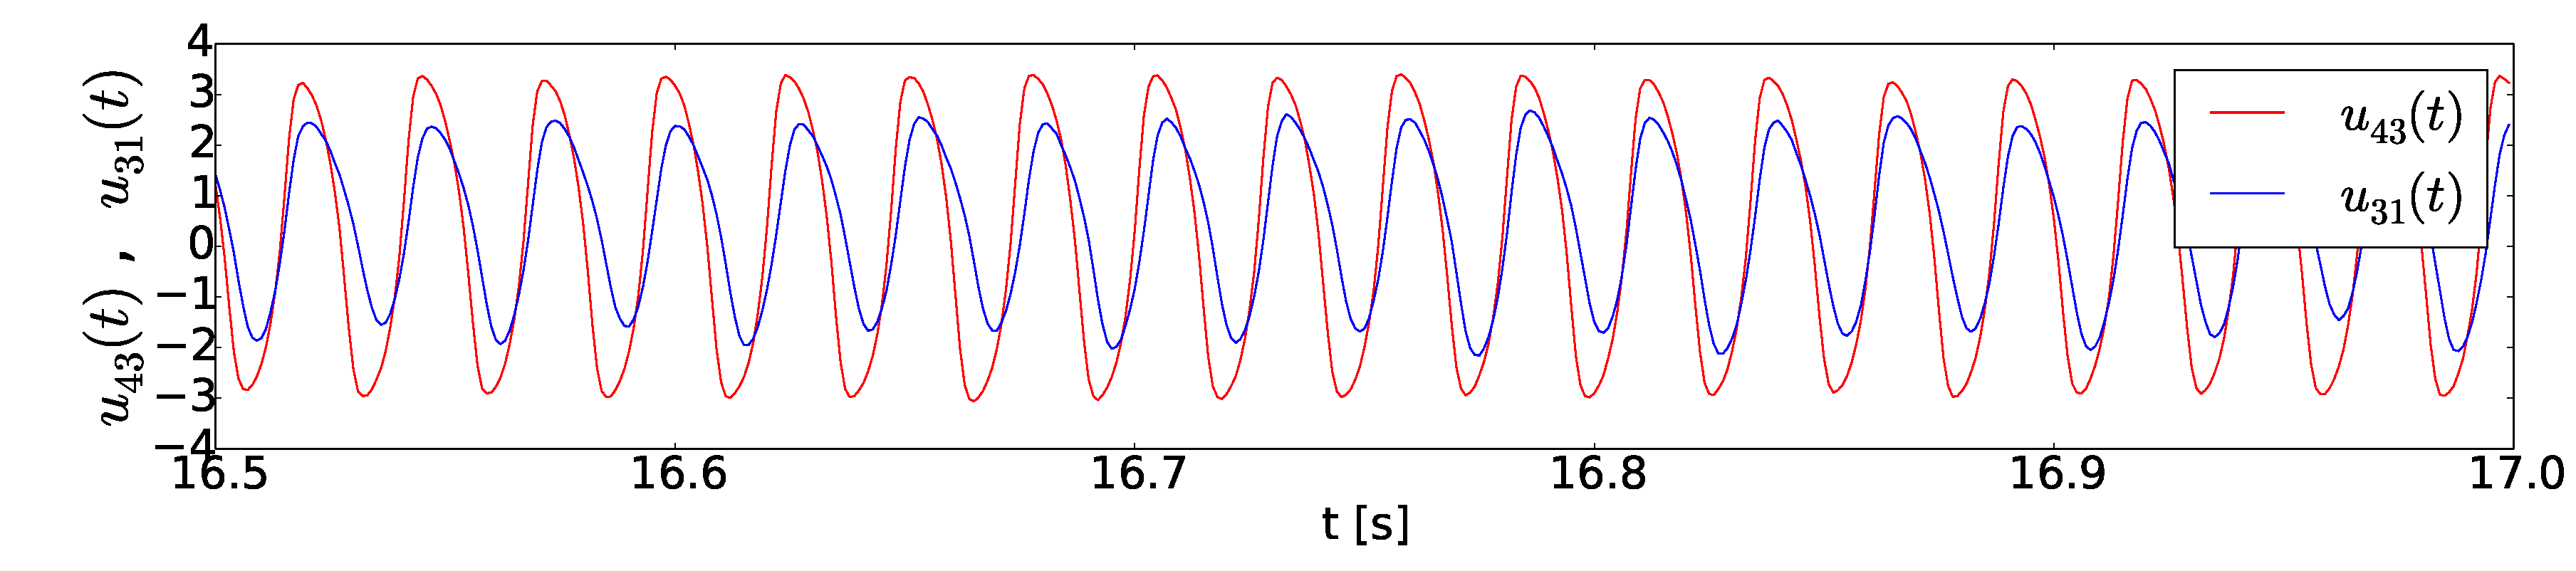
\includegraphics[width=\textwidth]{Figures/cor_ACM_sim_no_best.eps} 
   	 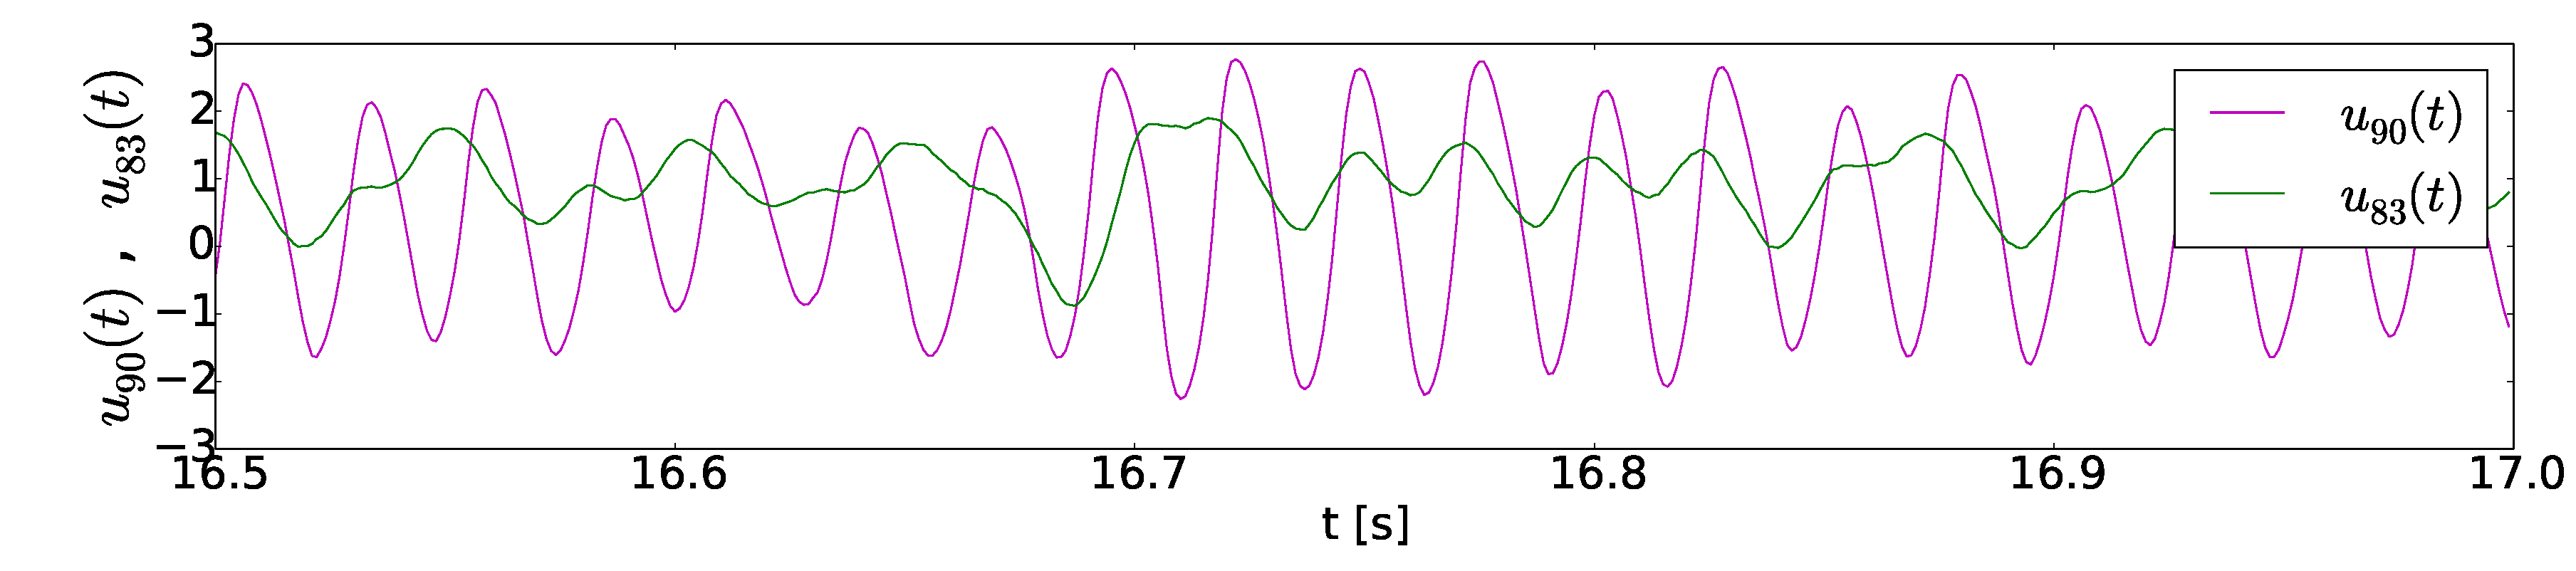
\includegraphics[width=\textwidth]{Figures/cor_ACM_sim_no_worst.eps} 

    \rule{35em}{0.5pt}
  \caption[Neural Activity Node Dynamics, ACM]{Simulated neuronal activity of highly (at top, $\rho_{43,31}=0.86$) and poorly (at bottom, $\rho_{90,83}=0.15$) correlated node couples. Both nodes are chosen from the simulated correlation matrix of ACM in previous figure ($c=0.3$, $v=6 [m/s]$, $r=0.50$).} 
    \label{fig:Neural Activity Node Dynamics, ACM}
 	
\end{figure} 




\begin{figure}[htbp]
 
  \centering
	 \includegraphics[width=0.8\textwidth]{Figures/FFT_ACM.eps} 
   	 %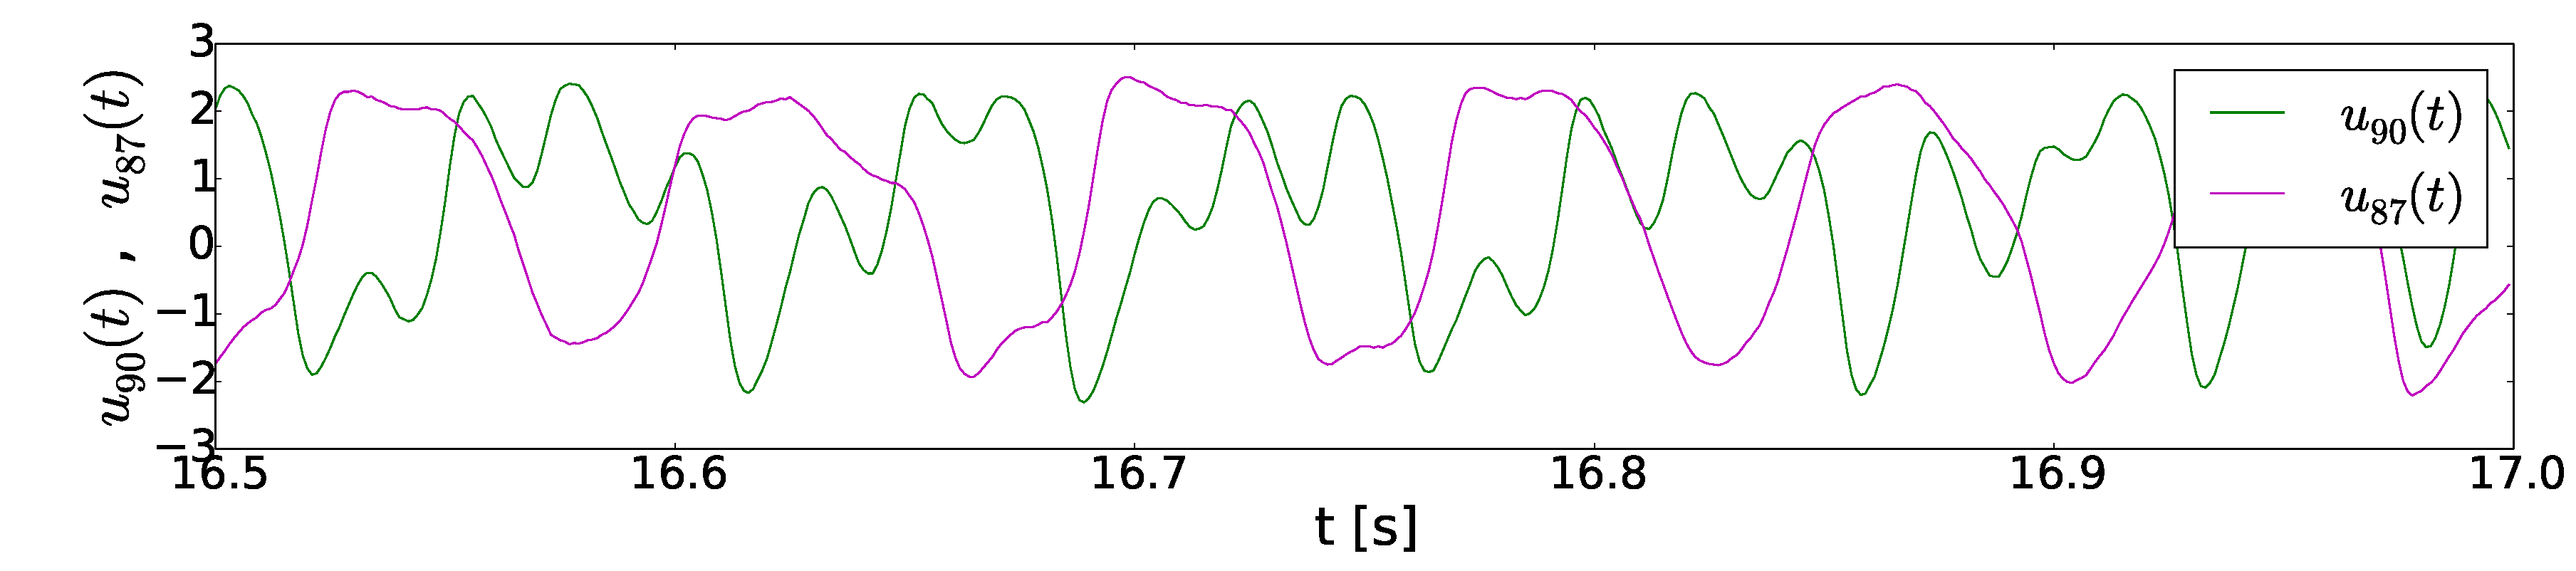
\includegraphics[width=\textwidth]{Figures/cor_FCM_sim_no_worst.eps} 

    \rule{35em}{0.5pt}
  \caption[3D Fourier Transform, FHN, ACM]{3D illustration of fast fourier transform of neuronal activity oscillations corresponding to $N=90$ nodes in ACM simulation with parameters given in Fig.3.6.} 
    \label{fig:3D Fourier Transform, FHN, ACM}
 	
\end{figure}  




\begin{figure}[htbp]
 
  \centering
    \includegraphics[width=0.49\textwidth]{Figures/PA_BOLD_FCM_v_7.eps} 
	\includegraphics[width=0.49\textwidth]{Figures/PA_BOLD_ACM_v_3.eps} 

	
    \rule{35em}{0.5pt}
  \caption[Parameter Analysis, BOLD]{Parameter analysis for BOLD simulations done with FCM (on the left, $v=7 [m/s]$) and ACM (on the right, $v=3 [m/s]$ ). Note that both simulation outcomes are correlated with only empirical FCM. }
  \label{fig:Parameter Analysis, BOLD}
 	
\end{figure} 



\begin{figure}[htbp]
 
  \centering
	 \includegraphics[width=0.49\textwidth]{Figures/cor_BOLD_FCM_sim.eps} 
   	 \includegraphics[width=0.49\textwidth]{Figures/cor_FCM_exp.eps} 

    \rule{35em}{0.5pt}
  \caption[Best correlated BOLD simulation, FCM]{Highly correlated BOLD simulation of FCM brain graph with $c=0.03$, $v=7 [m/s]$ and $r=0.66$ (on the left) and empirical FCM obtained from fMRI-BOLD. $\rho_{e,s} = 0.24$} 
    \label{fig:Best correlated BOLD simulation, FCM}
 	
\end{figure}  





\begin{figure}[htbp]
 
  \centering
	 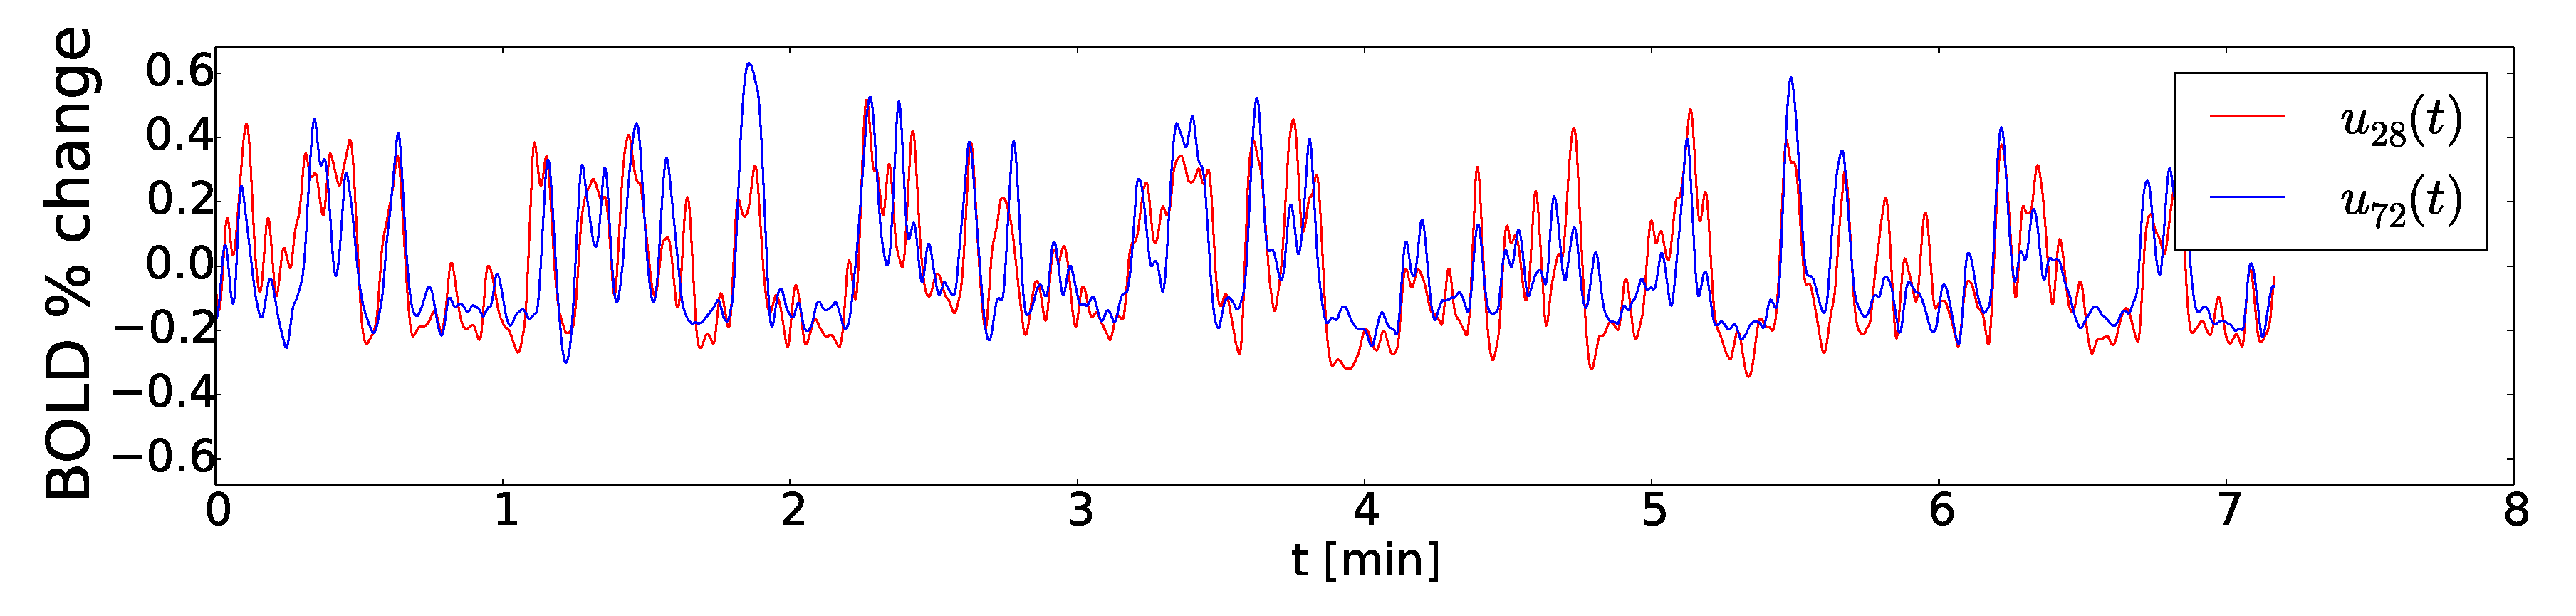
\includegraphics[width=\textwidth]{Figures/cor_BOLD_FCM_sim_no_best.eps} 
   	 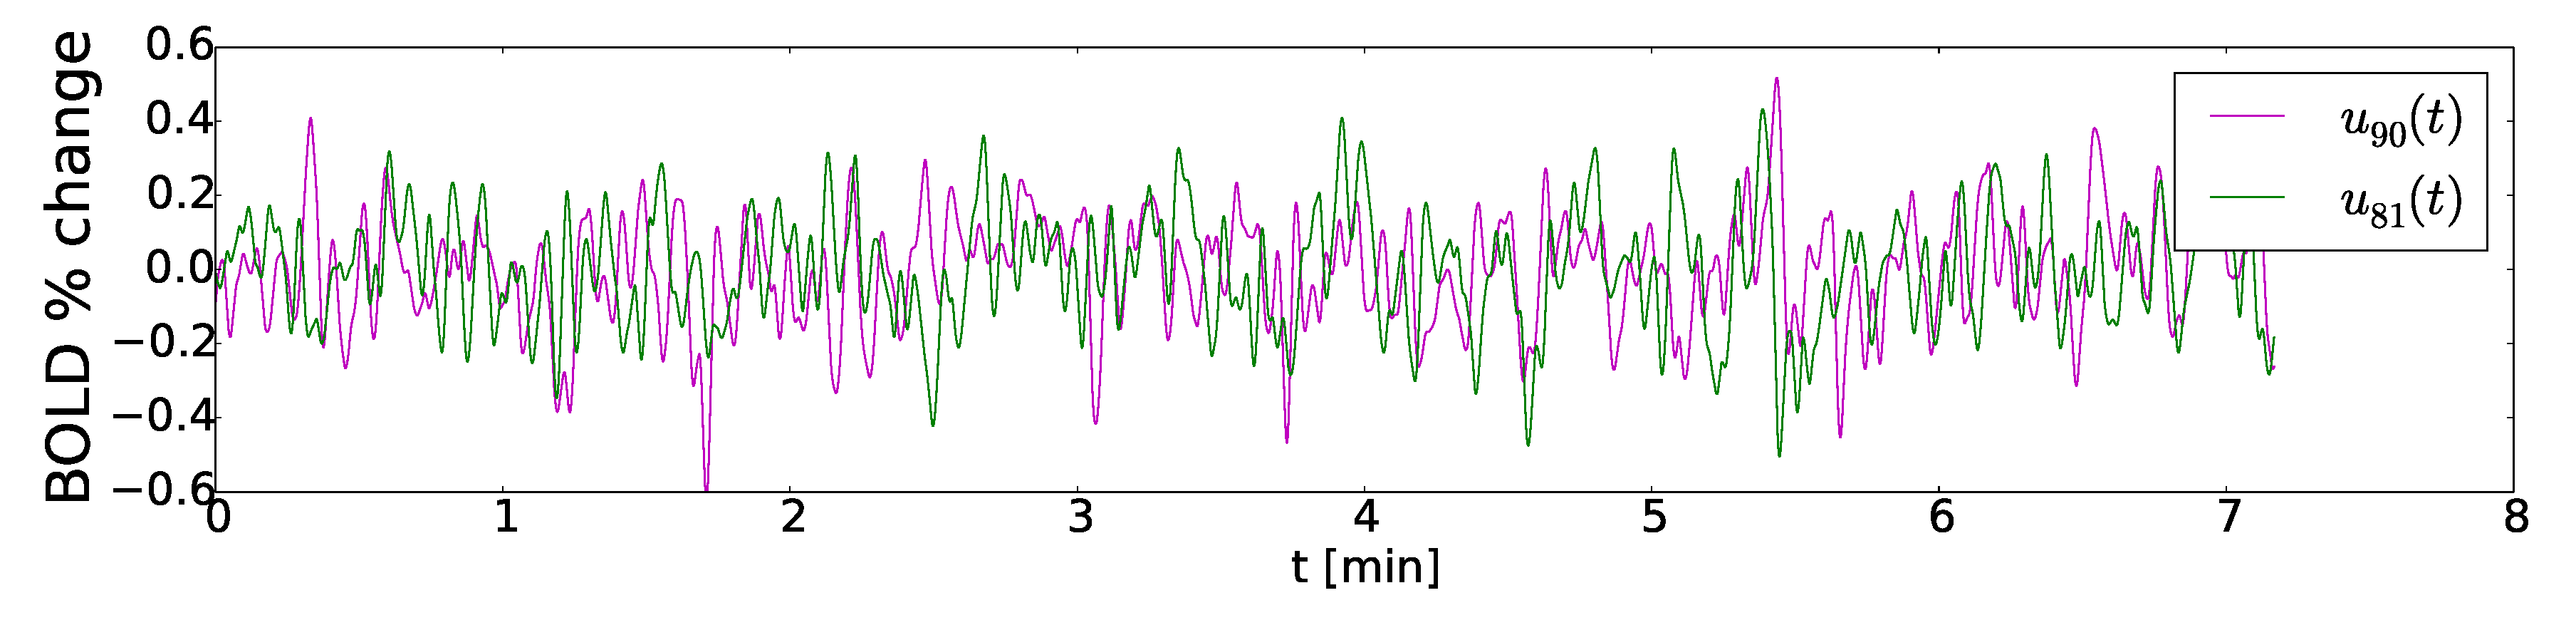
\includegraphics[width=\textwidth]{Figures/cor_BOLD_FCM_sim_no_worst.eps} 

    \rule{35em}{0.5pt}
  \caption[BOLD Activity Node Dynamics, FCM]{Simulated BOLD activity of highly (at top, $\rho_{28,72}=0.75$) and poorly (at bottom, $\rho_{90,81}=0.11$) correlated node couples. Both nodes are chosen from the simulated correlation matrix in previous figure ($c=0.03$, $v=7 [m/s]$, $r=0.66$).} 
    \label{fig:BOLD Activity Node Dynamics, FCM}
 	
\end{figure} 



\begin{figure}[htbp]
 
  \centering
	 \includegraphics[width=0.8\textwidth]{Figures/FFT_BOLD_FCM.eps} 
   	 %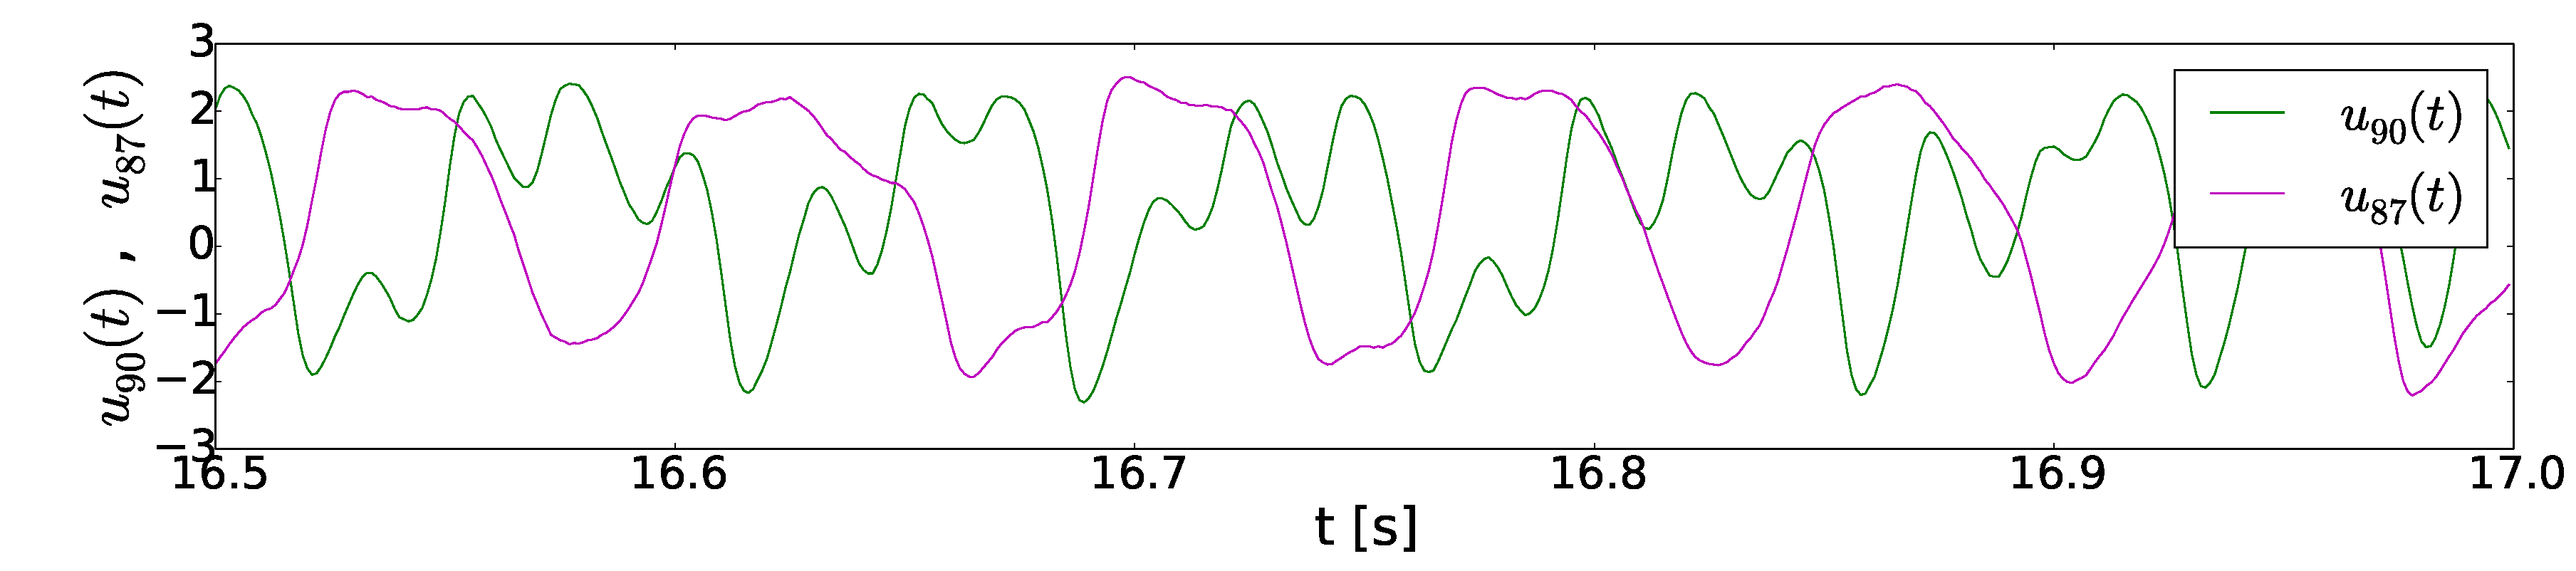
\includegraphics[width=\textwidth]{Figures/cor_FCM_sim_no_worst.eps} 

    \rule{35em}{0.5pt}
  \caption[3D Fourier Transform, BOLD, FCM]{3D illustration of fast fourier transform of BOLD activity slow oscillations corresponding to $N=90$ nodes in FCM simulation with parameters given in Fig.3.10.} 
    \label{fig:3D Fourier Transform, BOLD, FCM}
 	
\end{figure}  


\begin{figure}[htbp]
 
  \centering
	 \includegraphics[width=0.49\textwidth]{Figures/cor_BOLD_ACM_sim.eps} 
   	 \includegraphics[width=0.49\textwidth]{Figures/cor_FCM_exp.eps} 

    \rule{35em}{0.5pt}
  \caption[Best correlated BOLD simulation, ACM]{Highly correlated BOLD simulation of ACM brain graph with $c=0.03$, $v=3 [m/s]$ and $r=0.54$ (on the left) and empirical FCM obtained from fMRI-BOLD. $\rho_{e,s} = 0.22$} 
    \label{fig:Best correlated BOLD simulation, ACM}
 	
\end{figure}  




\begin{figure}[htbp]
 
  \centering
	 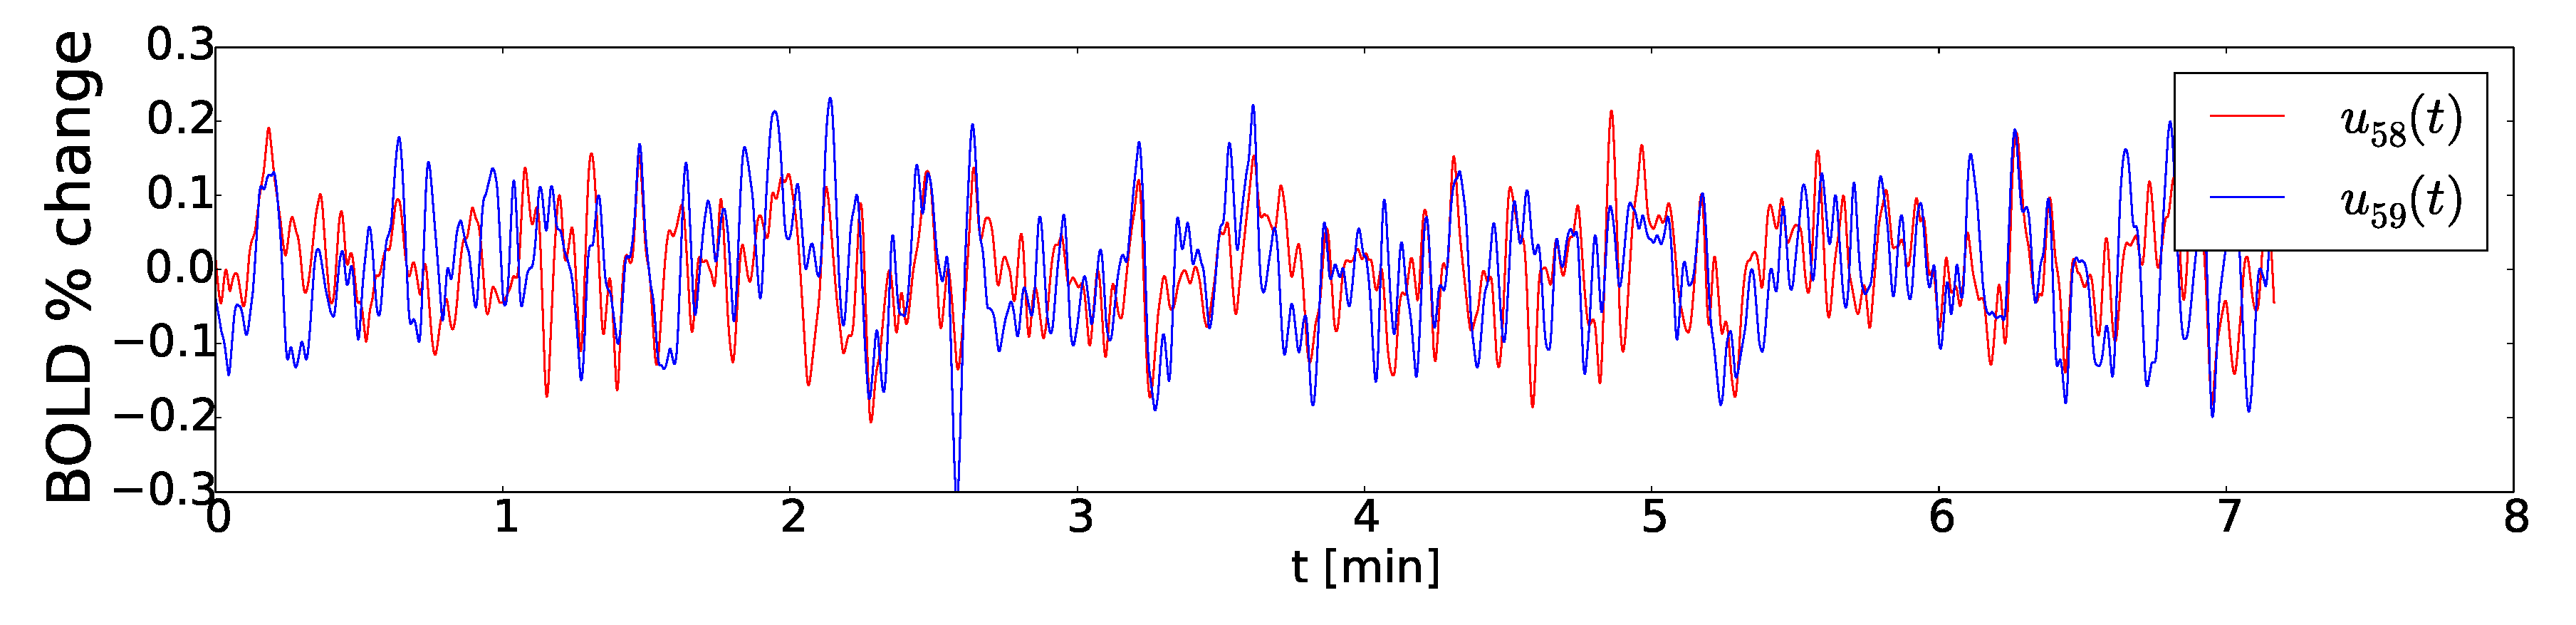
\includegraphics[width=\textwidth]{Figures/cor_BOLD_ACM_sim_no_best.eps} 
   	 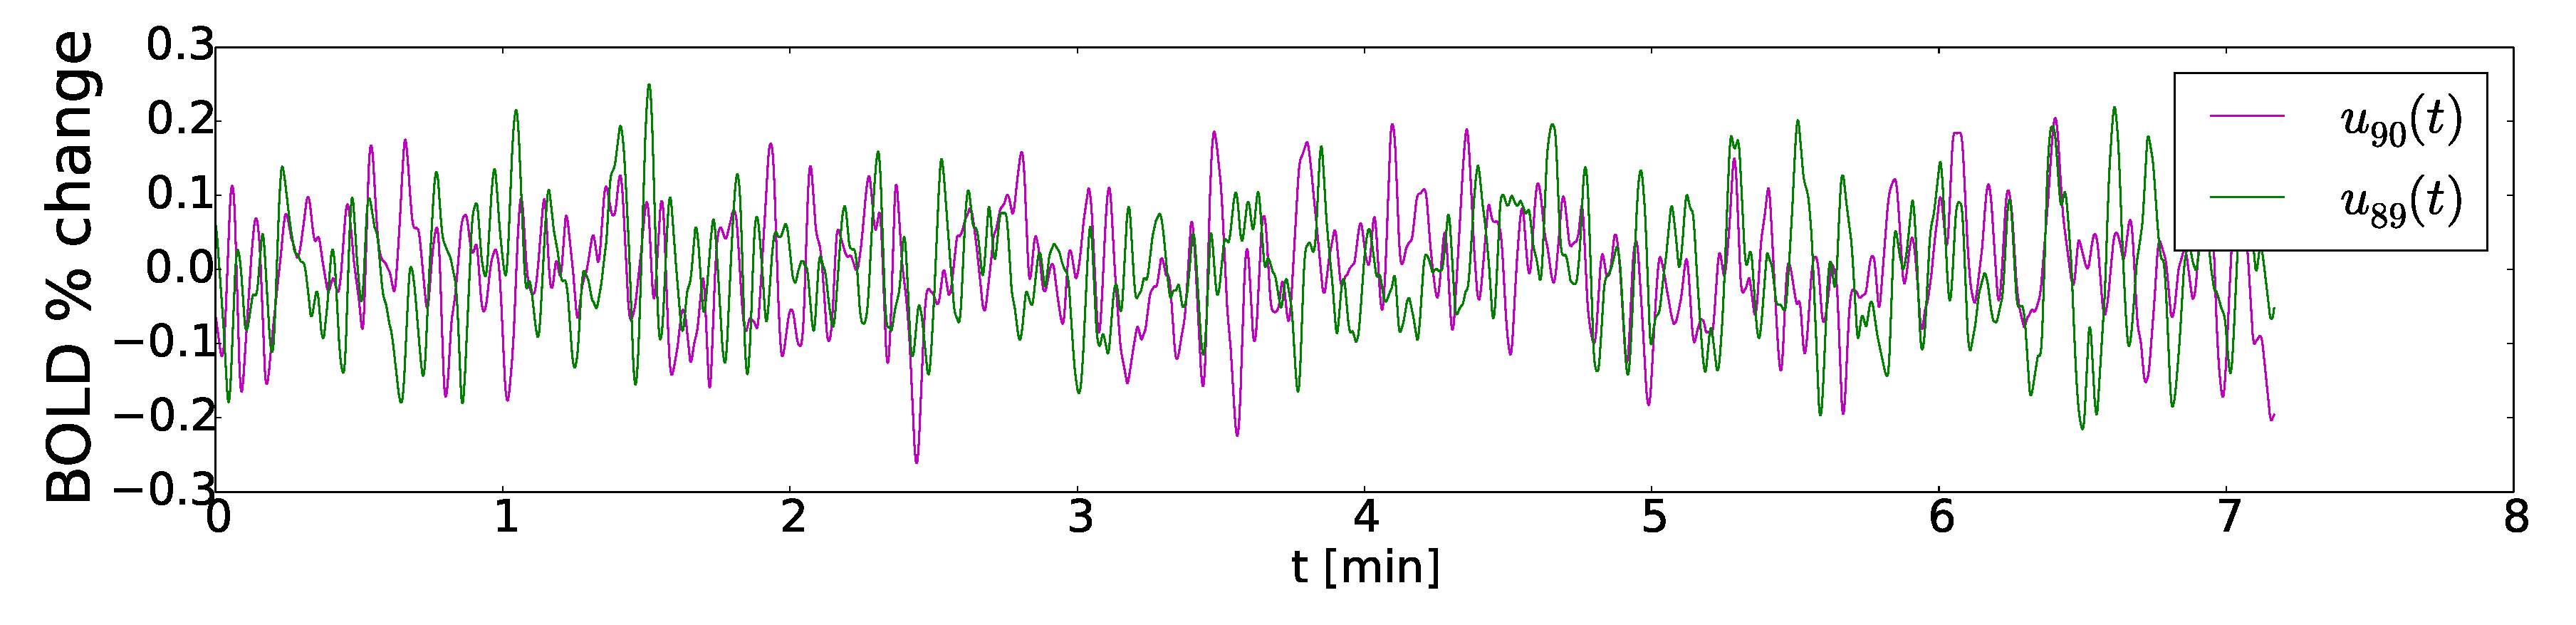
\includegraphics[width=\textwidth]{Figures/cor_BOLD_ACM_sim_no_worst.eps} 

    \rule{35em}{0.5pt}
  \caption[BOLD Activity Node Dynamics, ACM]{Simulated BOLD activity of highly (at top, $\rho_{58,59}=0.48$) and poorly (at bottom, $\rho_{90,89}=0.11$) correlated node couples. Both nodes are chosen from the simulated ACM correlation matrix in previous figure ($c=0.03$, $v=3 [m/s]$, $r=0.54$).} 
    \label{fig:BOLD Activity Node Dynamics, ACM}
 	
\end{figure} 





\begin{figure}[htbp]
 
  \centering
	 \includegraphics[width=0.8\textwidth]{Figures/FFT_BOLD_ACM.eps} 
   	 %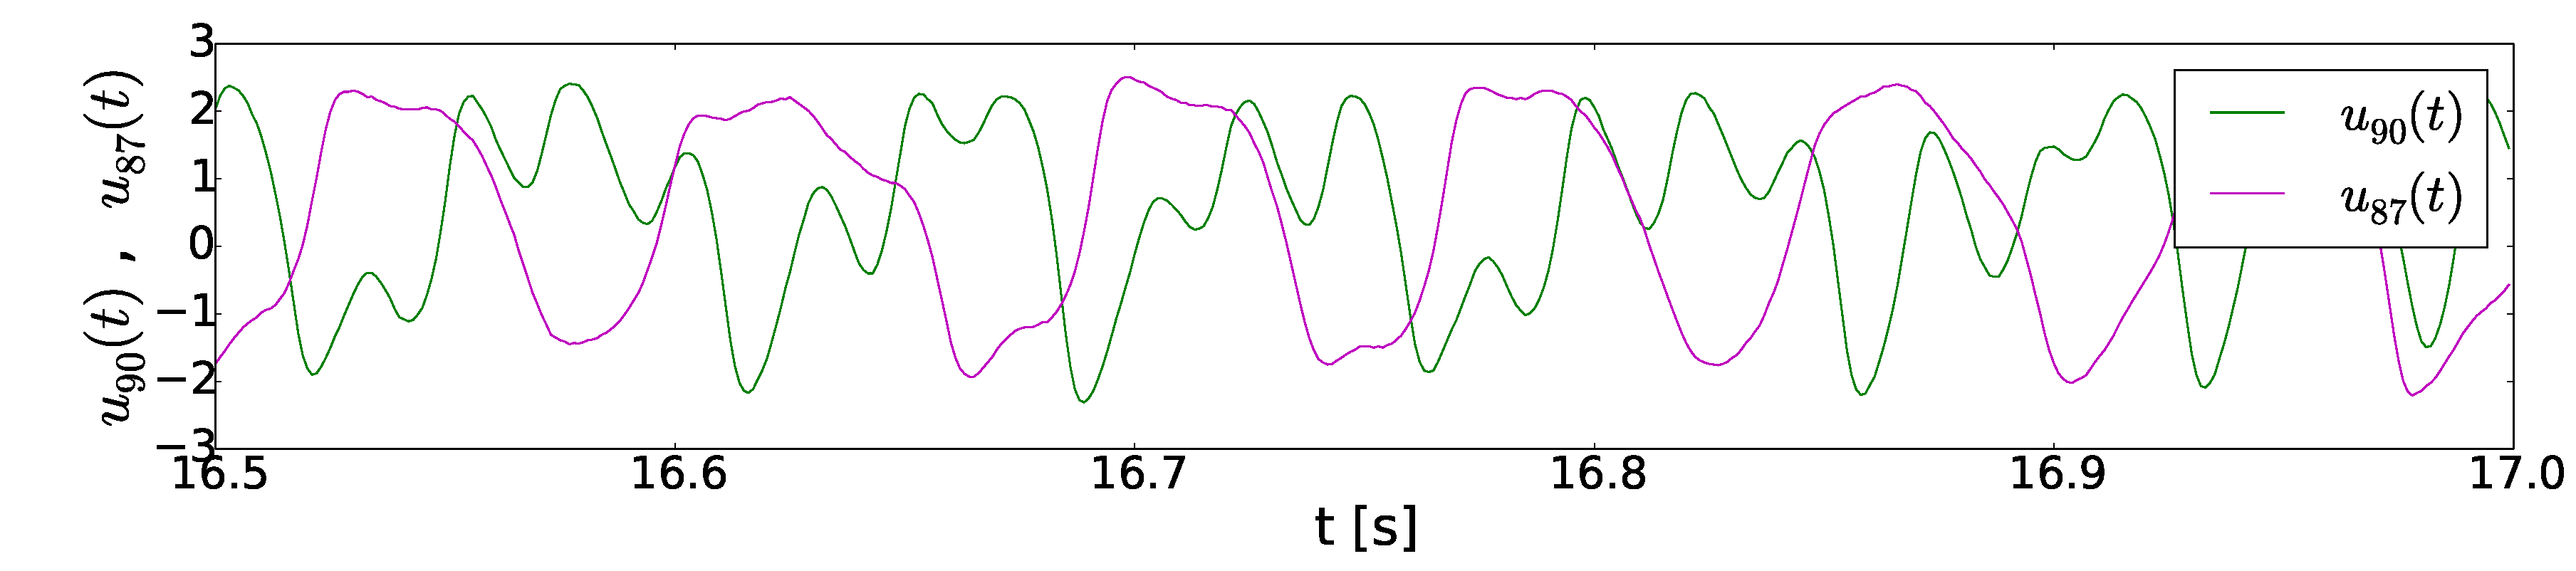
\includegraphics[width=\textwidth]{Figures/cor_FCM_sim_no_worst.eps} 

    \rule{35em}{0.5pt}
  \caption[3D Fourier Transform, BOLD, ACM]{3D illustration of fast fourier transform of BOLD activity slow oscillations corresponding to $N=90$ nodes in ACM simulation with parameters given in Fig.3.13.} 
    \label{fig:3D Fourier Transform, BOLD, ACM}
 	
\end{figure}  







